%%%%%%%%%%%%%%%%%%%%%%%%%%%%%%%%%%%%%%%%%%%%%%%%%%%%%%%%%%%%%%%%%%%%%%
% writeLaTeX Example: A quick guide to LaTeX
%
% Source: Dave Richeson (divisbyzero.com), Dickinson College
% 
% A one-size-fits-all LaTeX cheat sheet. Kept to two pages, so it 
% can be printed (double-sided) on one piece of paper
% 
% Feel free to distribute this example, but please keep the referral
% to divisbyzero.com
% 
%%%%%%%%%%%%%%%%%%%%%%%%%%%%%%%%%%%%%%%%%%%%%%%%%%%%%%%%%%%%%%%%%%%%%%
% How to use writeLaTeX: 
%
% You edit the source code here on the left, and the preview on the
% right shows you the result within a few seconds.
%
% Bookmark this page and share the URL with your co-authors. They can
% edit at the same time!
%
% You can upload figures, bibliographies, custom classes and
% styles using the files menu.
%
% If you're new to LaTeX, the wikibook is a great place to start:
% http://en.wikibooks.org/wiki/LaTeX
%
%%%%%%%%%%%%%%%%%%%%%%%%%%%%%%%%%%%%%%%%%%%%%%%%%%%%%%%%%%%%%%%%%%%%%%

\documentclass[10pt,landscape]{article}
\usepackage{amssymb,amsmath,amsthm,amsfonts}
\usepackage{multicol,multirow}
\usepackage{calc}
\usepackage{ifthen}
\usepackage{graphicx}
\usepackage{listings}
\usepackage{fancyvrb}
\usepackage[landscape]{geometry}
\usepackage[colorlinks=true,citecolor=blue,linkcolor=blue]{hyperref}


\ifthenelse{\lengthtest { \paperwidth = 11in}}
    { \geometry{top=.3in,left=.3in,right=.3in,bottom=.3in} }
  {\ifthenelse{ \lengthtest{ \paperwidth = 297mm}}
    {\geometry{top=1cm,left=1cm,right=1cm,bottom=1cm} }
    {\geometry{top=1cm,left=1cm,right=1cm,bottom=1cm} }
  }
\pagestyle{empty}
\makeatletter
\renewcommand{\section}{\@startsection{section}{1}{0mm}%
                                {-1ex plus -.5ex minus -.2ex}%
                                {0.5ex plus .2ex}%x 
                                {\normalfont\normalsize\bfseries}}
\renewcommand{\subsection}{\@startsection{subsection}{2}{0mm}%
                                {-1explus -.5ex minus -2ex}%
                                {0.2ex plus -1ex}%
                                {\normalfont\small\bfseries}}
\renewcommand{\subsubsection}{\@startsection{subsubsection}{3}{0mm}%
                                {-1ex plus -.5ex minus -.5ex}%
                                {0.2ex plus -1ex}%
                                {\normalfont\footnotesize\bfseries}}
\makeatother
\setcounter{secnumdepth}{0}
\setlength{\parindent}{0pt}
\setlength{\parskip}{0pt plus 0.5ex}
\graphicspath{ {./images/} }
% -----------------------------------------------------------------------

\title{CS2040s Cheatsheet Finals AY2022/2023 Semester 2}

\begin{document}

\raggedright
\footnotesize

\begin{center}
     \Large{\textbf{CS2109S Midterm Cheatsheet AY23/24 Sem 2 (Gavin)}} \\
\end{center}
\begin{multicols}{3}
\setlength{\premulticols}{1pt}
\setlength{\postmulticols}{1pt}
\setlength{\multicolsep}{1pt}
\setlength{\columnsep}{2pt}
\begin{scriptsize}

\subsubsection{Intelligent Agents}
\textbf{Agents} 
\begin{itemize}
  \item PEAS = Performance Measure, Environment, Actuators, Sensors
\end{itemize}
\textbf{Task Environment} 
\begin{itemize}
  \item Fully observable vs Partially observable
  \item Deterministic vs Stochastic vs Strategic 
  \\(Deterministic) Next state of the environment is completely determined by current state and agent action.
  \\(Strategic) Environment is deterministic except for actions of other agents.
  \item Episodic vs Sequential
  \item Static vs Dynamic vs Semi-dynamic
  \\(Semi-dynamic) Environment does not change with time, but agent's performance score does.
  \item Discrete vs Continuous
  \item Single Agent vs Multi-agent
\end{itemize}
\textbf{Agent Structure} 
\begin{itemize}
  \item Simple Reflex Agent:\\Selects action based on current percept, 
  ignoring percept history. Uses condition-action(if-then) rules
  \item Model-based Agent:\\Keep track of the part of
  the world it can’t see now. This internal state is updated
  through the transition model of the world (i.e. knowledge on how the world changes) and the sensor model,
  i.e. information from percepts.
  \item Goal-based Agent:\\In addition to tracking the state of
  the world, also track a set of goals, then pick the action
  that brings it closer to the goal.
  \item Ultility-based Agent:\\Uses an utility function to assign
  a score to any given percept sequence, i.e. an internalisation of the performance measure. If the utility function and the performance measure are aligned, then the agent
 will be rational.
  \item Learning Agent:\\Uses a performance element to select
  external actions, a critic to give feedback on how the
  agent is doing and how the performance element can be
  improved, a learning element responsible for making improvements, and a problem generator that suggests actions that will lead to new and informative experiences.
\end{itemize}


\subsection{Uninformed Searching}
\textbf{Representation invariant}\\Conditions that ensure abstract states have corresponding concrete states.

\includegraphics*[height=5.2cm, width=0.8\linewidth]{tree_search.png}

\textbf{Breadth-first search(BFS):}
\begin{itemize}
  \item Frontier: queue
  \item Time Complexity: $O(b^d)$
  \item Space Complexity: $O(b^d)$
  \item Complete? Yes if tree is finite
  \item Optimal? Yes, if step cost is same everywhere
\end{itemize}
\textbf{Uniform-cost search (UCS):}\\
\begin{itemize}
  \item Frontier: priority queue (path cost)
  \item Time Complexity: $O(b^{C*/\epsilon})$
  \item Space Complexity: $O(b^{C*/\epsilon})$
  \item Complete? Yes if $\epsilon > 0$ and $C*$ finite
  \item Optimal? Yes, if $\epsilon > 0$
\end{itemize}
$C*$: Cost of optimal solution; $\epsilon$: min edge cost.\\
Note: Goal-test is done after popping from frontier instead of goal-testing next state.\\
\textbf{Depth-first search(DFS):}
\begin{itemize}
  \item Frontier: stack
  \item Time Complexity: $O(b^m)$
  \item Space Complexity: $O(bm)$
  \item Complete? No. Possibility of infinite loops with infinite trees
  \item Optimal? No
\end{itemize}
\textbf{Depth limited search(DLS):} DFS with limited search depth
\begin{itemize}
  \item Time Complexity: $b^0 + b^1 + \ldots + b^l = O(b^l)$
  \item Space Complexity: $O(bl)$
  \item Complete? No
  \item Optimal? No
\end{itemize}

\textbf{Iterative deepening search(IDS):} Do DLS with increasing $l$
\begin{itemize}
  \item Time Complexity: $O(d+1)b^0 + db^1 + (d-1)b^2 + \ldots + 2b^{d-1} + b^d = O(b^d)$
  \item Space Complexity: $O(bd)$
  \item Complete? Yes
  \item Optimal? Yes, if step cost is same everywhere
\end{itemize}
\textbf{Bidirectional search:}: Combine search from forward and backwards
\begin{itemize}
  \item Time Complexity: $ 2 * O(b^{d/2}) < O(b^d)$
\end{itemize}
\textbf{Graph search:}
\begin{itemize}
  \item Use a set to keep track and avoid expanding visited states.
  \item Version 1: If next state visited: continue. Add to frontier and visited in the end of action loop.
  \\ Expand less states, may skip states with less cost
  \item Version 2: After popping from frontier, immediately goal-test $\rightarrow$ visited-check: continue $\rightarrow$ visited.add(state)
  \\ Expand more states, will not skip states with less cost
\end{itemize}

\subsection{Informed Searching}
\textbf{Greedy best first search:}\\
Pick a node n from the frontier with minimum value of an
 evaluation function $f(n) = h(n)$. If goal state, return it, else expand to add its child nodes to the frontier. Child nodes are
 only added if they are unvisited or previously visited with
 a higher path cost.
 \begin{itemize}
  \item Time Complexity $O(b^m)$
  \item Space Complexity: $O(b^m)$
  \item Complete? No
  \item Optimal? No
\end{itemize}

\textbf{A* search:}\\
This is a Best-First Search that uses the evaluation function $f(n) = g(n) + h(n)$, where $g(n)$ is the path cost from
 the initial node to node n.
 Assuming all action costs are $> \epsilon> 0$ and that state space
 is finite, $A*$ search is complete. If there are infinitely many
 nodes with $f(n) \leq f(goal)$, then it is not complete. Time
 and space complexities are both exponential \textbf{$O(bd)$} for a
 poor heuristic. Whether it is cost-optimal depends on certain properties of the heuristic:
 
 \begin{itemize}
  \item \textbf{Admissibility}. Never overestimates the cost to reach a
  goal, i.e. optimistic $h(n) \leq h^*(n)$. If $h(n)$ is admissible, then $A^*$ using
  tree-like search is cost-optimal.
  \item \textbf{Consistency}. Stronger than admissibility. $h(n)$ is consistent if, for every node n and every successor $n'$ of $n$
  generated by an action $a$, we have $h(n) \leq c(n,a,n') +
  h(n')$, i.e. triangle inequality. If $h(n)$ is consistent, then
  $A*$ using graph search is cost-optimal.\\\textbf{A consistent heuristic is admissible}, but not the other way around.
  \item \textbf{Dominance}. If $h_2(n) \geq h_1(n)$ for all $n$, then $h_2$ dominates $h_1$. 
  More dominant heuristics are better for search.
\end{itemize}

A problem with fewer restrictions on actions is called a \textbf{relaxed problem}.
The cost of an optimal solution to a relaxed problem is an admissible heuristic for the original problem.\\

\textbf{Iterative Deepening A* (IDA*)}: Use iterative deepening search. Cutoff using f-cost $f(n) = g(n) + h(n)$ instead of depth.\\
\textbf{Simplified memory-bounded A* (SMA*)}: Drop the nodes with worst f-cost in frontier when memory is full.

\subsection{Local Search}
\textbf{Path is not important, state is the solution.}\\
Consists of initial state, goal test, successor function(heuristic or objective function)

\textbf{Hill climbing algorithm}\\
Find local maxima by travelling to neighbouring states with
 the highest value, and terminating when no neighbour has
 a higher value. Easy objective function is to negate the
 heuristic function.
 This algorithm suffers from local maxima (i.e. non-global
 maximum), ridges (sequence of local maxima), plateaus
 (sequence of same values, but is local maxima) and shoulders (same values, but progress is possible). 
 \\Solutions are:
 \begin{itemize}
  \item Sideways Move. We do a limited number of consecutive sideways move, in hopes that the plateau is really a
  shoulder.
  \item Stochastic Hill Climbing. Chooses a random uphill
  move, with probabilities based on the steepness of the
  move.
  \item First-choice Hill Climbing. Randomly generate successors until one is better than the current state. Useful
  when a state has e.g. thousands of successors.
  \item Random-Restart Hill Climbing. Perform a fixed
  number of steps from some randomly generated initial
  steps, then restart if no maximum found.
 \end{itemize}

 \textbf{Simulate annealing}\\
 Basically, randomly pick a next move. If it's a better state,
 go for it, else accept it with a probability less than 1, and
 this probability decreases exponentially with the “badness”
 of the move. Idea is to escape local maxima by allowing
 some random moves once in a while. \\
 If T decreases slowly enough, simulated annealing will find a global optimum with high probability.

 \textbf{Local beam search}\\
 Pick $k$ random initial states \textbf{deterministically}, then generate their successors.
 If goal is found, terminate, else pick the $k$ best successors
 and repeat. Similar to $k$ random restarts but information
 is shared. It may suffer from a lack of diversity if the $k$
 states start to cluster. \textbf{Stochastic beam search} alleviates this problem by choosing $k$ successors with \textbf{probability}
 proportional to their value.

\textbf{Genetic algorithm}\\
$\text{Population} \underbrace{\rightarrow}_{\text{Fitness Function}} \text{Selection} \rightarrow \text{Cross-Over} \rightarrow \text{Mutation} \rightarrow \text{New Population}$

%\newpage

\subsection{Adversarial Search and Games}
The most commonly studied games are deterministic, two-player, turn-taking, perfect information, zero-sum games.
Perfect information just means fully observable, and zero 
sum means that there is no “win-win” situation.

\textbf{Minimax algorithm}\\
Opponent has to behave optimally for algorithm to work.

% Insert image here
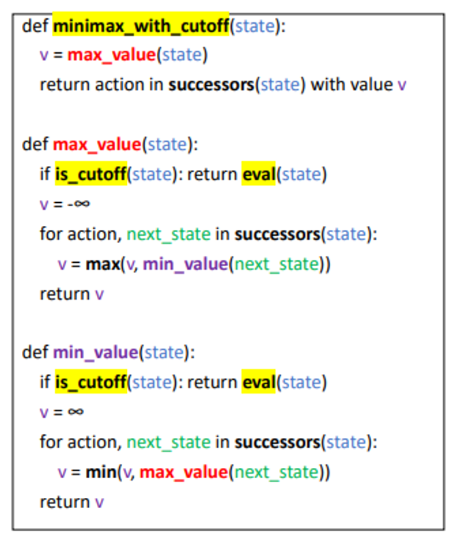
\includegraphics[height= 5cm, width=0.4\linewidth]{minimax_cutoff.png}
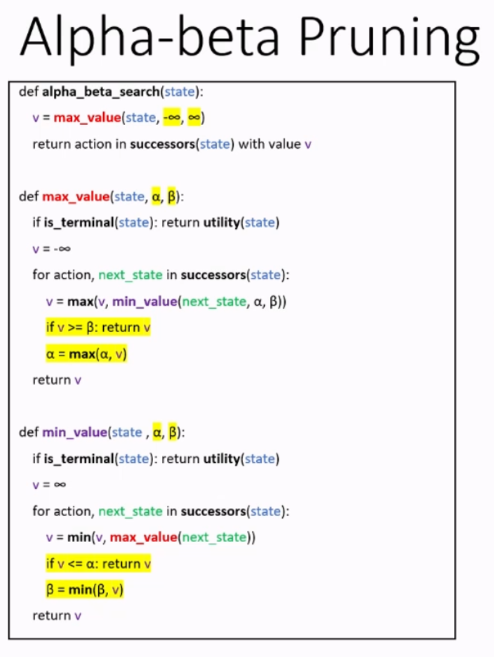
\includegraphics[height= 5cm, width=0.5\linewidth]{alpha_beta_pruning.png}
\\ $\textbf{is\_cutoff()}$ returns true if state is terminal or cutoff (depth/time) is reached.
\\ $\textbf{eval()}$ returns utility for terminal states, and heuristic values for non-terminal states.

\textbf{Alpha-beta pruning}\\
\begin{itemize}
  \item Max node: only $v$ and $\alpha$ is modified
  \item Min node: only $v$ and $\beta$ is modified
  \item When modifying $\alpha$, find max of previous $\alpha$ and $\beta$ values.
  \item When modifying $\beta$, find min of previous $\alpha$ and $\beta$ values.
  \item Prune when $\alpha \geq \beta$
  \item Remember to update $\alpha$ and $\beta$ values of parent when recursing back upwards.
  \item Good move ordering improves effectiveness of pruning. Perfect ordering: $O(b^{m/2})$
\end{itemize}

\textbf{Optimizing search}: Transposition table, pre-computation of best moves.

\subsection{Machine Learning}
In supervised learning, we assume that y is generated by a true mapping function $f : x \rightarrow y$. 
We want to find hypothesis $h : x \rightarrow \hat{y}$ (from hypothesis class H), s.t $h \approx f$
given a training set ${(x_1, f(x_1)), \ldots, (x_N, f(x_N))}$\\
\textbf{Classification}: Output is one of a finite set of values.\\
\textbf{Regression:} Output is a number.\\
Types of Feedback:
 \begin{itemize}
  \item Supervised Learning. Agent observes input-output
  pairs and learns a function that maps from input to output.
  \item Unsupervised Learning. Agent learns patterns in the
  input without any explicit feedback. Most common task
  is clustering.
  \item Reinforcement Learning. Agent learns from a series
  of reinforcements: rewards and punishments.
\end{itemize}

\textbf{Regression: Error}\\
Let $\hat{y_i} = h(x_i)$ (prediction) and $y_i = f(x_i)$ (actual)
\begin{itemize}
  \item $\text{Mean Absolute Error} = \frac{1}{N} \sum_{i=1}^{N} | \hat{y_i} - y_i |$
  \item $\text{Mean Squared Error} = \frac{1}{N} \sum_{i=1}^{N} (\hat{y_i} - y_i)^2$
\end{itemize}
\textbf{Classification Correctness and Accuracy}\\
\begin{itemize}
  \item $\text{Accuracy} = \frac{1}{N} \sum_{i=1}^{N} 1_{\hat{y_i} = y_i}$
\end{itemize}

\textbf{Classification: Confusion Matrix}\\
\begin{itemize}
  \item $\text{Accuracy} = \frac{TP + TN}{TP + FN + FP + TN}$
  \item $\text{Precision} = \frac{TP}{TP + FP}$ (Maximise this if FP is costly)
  \item $\text{Recall} = \frac{TP}{TP + FN}$ (Maximise this if FN is costly)
  \item $\text{F1 Score} = \frac{2}{\frac{1}{Precision} + \frac{1}{Recall}}$
\end{itemize}

\subsubsection*{Decision Trees}
\includegraphics*[height= 4cm, width=0.8\linewidth]{decision_tree_learning.png}

\textbf{Entropy}\\
\begin{itemize}
  \item $\text{Entropy} = - \sum_{i=1}^{n} p_i \log_2 (pi)$
  \item $\text{Remainder} = - \sum_{i=1}^{v} \frac{p_i + n_i}{p+n} I(\frac{p_i}{p_i + n_i}, \frac{n_i}{p_i + n_i})$
  \item $\text{Information Gain(A)} =  I(P_1, P_2, \ldots, P_n) - remainder(A)$
  \item Formulas can and should be extended when more than 2 categories are involved.
  \item $\text{Split Information} = - \sum_{i=1}^{d} \frac{|E_i|}{E} \log_2 \frac{|E_i|}{E}$
  \item $\text{Gain Ratio} = \frac{IG(A)}{Split \space Information(A)}$ (Use on attributes with many values)
\end{itemize}

\includegraphics*[height=5cm, width=0.45\linewidth]{binary_entropy_table.png}
\includegraphics*[height=5cm, width=0.5\linewidth]{log_base2_chart.png}

\textbf{Notes:}\\
- When dealing with Attributes of differing cost: Use Cost-Normalised Gain to ultilise low-cost attributes where possible.\\
- Continuous-valued attributes should be partitioned into discrete set of intervals to use decision trees.\\
- When dealing with missing values, you can assign most common value (with same output), drop the attribute, use probability, drop the row and so on.

\textbf{Pruning:}\\
\begin{itemize}
  \item \textbf{Occam's Razor}: Prefer short/simple hypothesis, hypothesis that fits are unlikely to be coincidence.
  \item min-sample: each node should have minimum around of values.
  \item max-depth: limit the depth of the decision tree.
  \item Pruning can be propagated upwards with majority combination.
\end{itemize}


\end{scriptsize}

\end{multicols}

\end{document}